\htwo{Implementierung von Docker und Nginx}
\sectionauthor{Johannes Polzer} 

Aufgrund der unterschiedlichen Anforderungen, wurde sowohl für die Entwicklung, als auch für die Produktion eine "docker-compose" YAML-Datei erstellt. 
Dadurch ist es möglich, dass in der Produktion der TypeScript-Code optimiert ist und damit kleinere Dateien auf den Client geladen werden müssen. 
Andererseits können auch Funktionen für die Entwicklung genutzt werden, wie das automatische neu Laden der Seite beim Speichern von Änderungen.

\hthree{Docker bei der Entwicklung}

Zunächst wurde für die Entwicklung eine separate NGINX-Konfiguration (Siehe Code \ref{code:nginxDevConf}) erstellt, die den Entwicklungsserver, der von Vite betrieben wird, an den Client weitergibt.

\css[code:NginxDevConf]{code/Nginx/dev.conf}{NGINX-Konfiguration für die Entwicklung}

Um das Gesamtprojekt bereitzustellen, werden vier verschiedene Docker-Container gestartet.

Der erste ist die "MariaDB"-Datenbank, die alle Daten speichert. Der zweite ist die "API", die die Daten verwaltet und über unseren dritten Container, einen "NGINX"-Webserver, an die Webclients weiterleitet. Die Website selbst wird vom "Vite"-Entwicklungsserver bereitgestellt, der den vierten Container darstellt. 

\begin{figure}[H]
    \centering
    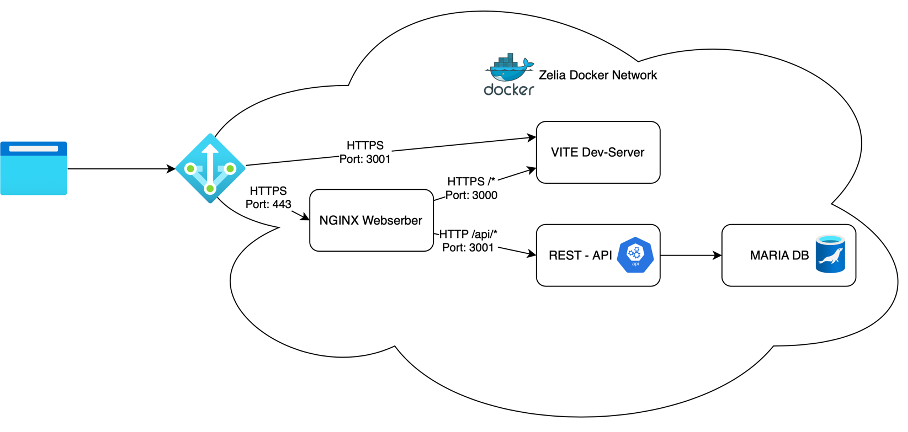
\includegraphics{media/Docker/DevNetwork.png}
    \caption{Docker-Netzwerk für die Entwicklung}
\end{figure}

Um das Datenbankschema aufzubauen und "Dummy"-Daten einzufügen, können SQL-Skripte im Verzeichnis /docker-entrypoint-initdb.d/ angelegt werden. Dort werden sie beim Start des Docker-Containers in alphabetischer Reihenfolge ausgeführt. Daher wurden sie mit Zahlen beginnend benannt, um die Reihenfolge festzulegen.

Um "Secrets" wie das Passwort zur Datenbank zu schützen, werden sie aus Umgebungsvariablen übernommen. Damit es nicht notwendig ist, die "Environment"-Variablen jedes Mal manuell zu setzten, ist es bei Docker möglich, eine "Env"-Datei anzugeben, die alle Umgebungsvariablen speichert. 

\css{code/Docker/dev.yaml}{Docker-YAML für die Entwicklung}

\hthree{Docker in der Produktion}

Für die Produktion werden die Webseiten für den Client einmal erstellt und als statische Dateien von NGINX bereitgestellt. 
Daher wird der Docker-Container für den Entwicklungs-Vite-Server nicht benötigt. 
Um die Daten der Datenbank zu persistieren, werden sie in einem Docker-Volume gespeichert. 

Allerdings werden für die Produktion Docker-Images für die Rest API und den NGINX Webserver gebaut. Dabei werden alle Abhängigkeiten installiert und der TypeScript-Code wird zu Javascript-Code transpiliert. Dadurch muss zum Starten nur mehr ein Container mit dem erstellten Image erzeugt werden. 
Dabei ist es wichtig, dass alle erforderlichen Umgebungsvariablen gesetzt sind.

\begin{figure}[H]
    \centering
    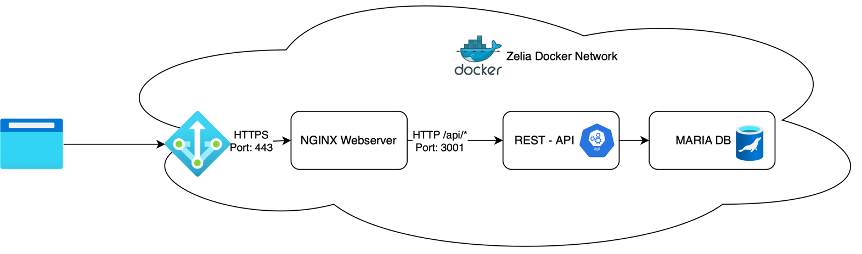
\includegraphics{media/Docker/ProdNetwork.png}
    \caption{Docker-Netzwerk für die Produktion}
\end{figure}

Da alle Container innerhalb des \ZELIA-Docker-Netzwerks liegen, ist es nicht möglich, dass direkt auf die Datenbank zugegriffen werden kann, da der einzig offene Port auf den NGINX Webserver verweist. 

\css{code/Nginx/prod.conf}{NGINX-Konfiguration für die Produktion}

% todo: Add docker-compose.yml
